% Selbst erstelltes Mockup einer Wetter-App mit Entscheid für den Schulweg (Velo oder Tram).
% Ersetzt den früheren Screenshot if-elif-else-weather.png (Quelle nicht belegt).
% Emojis: Noto Color Emoji via \emoji{} (Apache License 2.0).
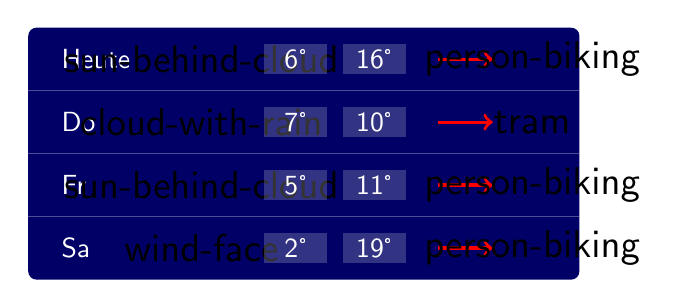
\begin{tikzpicture}[x=1cm, y=-.8cm, font=\sffamily,
		temp/.style={fill=white, fill opacity=.2, text opacity=1, text=white, minimum width=.8cm, inner sep=2pt}]
	\fill[rounded corners=3pt, blue!40!black] (0,-.5) rectangle (7,3.5);
	% Trennlinien zwischen den Tagen
	\foreach \y in {.5,1.5,2.5} {
			\draw[white, opacity=.3] (0,\y) -- (7,\y);
		}
	% Tag / Wetter / Tiefst- und Höchsttemperatur / Entscheid
	\foreach \tag/\wetter/\tmin/\tmax/\weg [count=\y from 0] in {
			Heute/sun-behind-cloud/6/16/person-biking,
			Do/cloud-with-rain/7/10/tram,
			Fr/sun-behind-cloud/5/11/person-biking,
			Sa/wind-face/2/19/person-biking} {
			\node[anchor=west, text=white] at (.3,\y) {\tag};
			\node[scale=1.4] at (2.2,\y) {\emoji{\wetter}};
			\node[temp] at (3.4,\y) {\tmin\textdegree};
			\node[temp] at (4.4,\y) {\tmax\textdegree};
			\draw[->, very thick, red] (5.2,\y) -- (5.9,\y);
			\node[scale=1.4] at (6.4,\y) {\emoji{\weg}};
		}
\end{tikzpicture}
